\documentclass[12pt,a4paper]{ctexart}

% --- Packages ---
\usepackage{amsmath,amsfonts,amssymb}
\usepackage{graphicx}
\usepackage{booktabs}
\usepackage{multirow}
\usepackage{tabularx}
\newcolumntype{Y}{>{\centering\arraybackslash}X}
\usepackage{geometry}
\usepackage{setspace}
\usepackage{caption}
\usepackage{subcaption}
\usepackage[numbers,sort&compress]{natbib}
\usepackage{hyperref}
\usepackage{cleveref}
\usepackage{xcolor}
\usepackage{authblk}
\usepackage{quoting}

% --- Setup ---
\geometry{left=2.5cm, right=2.5cm, top=2.5cm, bottom=2.5cm}
\setstretch{1.5}
\hypersetup{
    colorlinks=true,
    linkcolor=blue,
    filecolor=magenta,      
    urlcolor=cyan,
    citecolor=blue,
}

\title{传统产业集群韧性演化与地方政府制度响应——以高阳毛巾集群为例}
\author[1]{作者姓名}
\affil[1]{作者单位}
\date{\today}

\begin{document}

\maketitle

\begin{abstract}
随着全球经济步入以逆全球化、环保规制和结构性市场变迁为特征的转型期，传统劳动密集型产业集群面临外部冲击带来的适应性挑战。本文以中国高阳县毛巾产业集群（2000--2024）为研究对象，采用混合方法纵向单案例研究设计，探讨地方政府政策干预与产业集群韧性的协同演化机制。首先，利用BERTopic模型对25年的地方政府工作报告进行全文本建模，刻画政策焦点的时序变迁，并引入多重安慰剂主题检验确保NLP指标的区分效度；其次，运用合成控制法（SCM）和中断时间序列分析（ITS），基于高阳县及保定市24个区县的面板数据，对环保基建冲击的企业存活效应进行多源三角验证。研究发现，高阳集群的韧性演化经历了从"规模扩张"到"底盘韧性"、最终向"价值韧性"的递进过程，地方政府的敏捷政策注意力转移在其中发挥了关键的支撑作用。本文通过量化政策注意力（而非制度支出）并引入微观成本视角，对区域经济韧性文献进行了实证补充。

\vspace{0.5cm}
\noindent\textbf{关键词：} 区域经济韧性；产业集聚；BERTopic；合成控制法；中断时间序列；制度供给
\end{abstract}

\newpage
\section{引言}
\label{sec:intro}

当前，全球经济格局已从高速全球化阶段步入以不确定性、复杂性和突发性为特征的转型期 \cite{Tooze2022}。对于广大发展中国家的传统劳动密集型产业集群而言，这一时代背景意味着它们必须面对一系列外部冲击：人口红利减弱、国内环保规制收紧、以及国际贸易环境的变化 \cite{Gong2022}。曾经依赖低成本代工（OEM）模式在“微笑曲线”底部发展的制造基地，正面临严峻的转型压力。在这些结构性变革中，部分集群因无法承担新增成本而出现衰退；而另一些集群则展现出一定的适应力，实现了产业链的升级。这种差异引出了一个关键问题：\textit{在外部冲击下，传统产业集群是如何演化其韧性的？在这一过程中，地方政府的制度供给发挥了怎样的作用？}

区域经济韧性（Regional Economic Resilience, RER）作为解释区域经济系统抵御、吸收外部冲击并恢复或转型能力的概念，近年来在经济地理学和区域研究领域受到关注 \cite{Martin2012, Boschma2015}。然而，现有文献在探讨集群韧性时存在两方面局限。其一，经验研究多聚焦于发达国家的高新技术或先进制造集群，对发展中国家传统产业集群的关注相对不足 \cite{Li2022}。其二，主流的宏观计量分析往往侧重于考察产业结构（如相关多样化）对韧性的影响，对地方政府应对外部冲击时的政策组合（Policy Mixes）及其微观传导机制的探讨有待深入 \cite{Rothgang2024, Bachtler2024}。当面临系统性的监管要求或市场波动时，单纯依靠市场机制调节可能存在协调失灵；此时，地方政府的政策干预——如通过提供公共物品来承担部分外部成本并引导结构转型——可能成为影响集群韧性演化方向的重要因素。

为弥补上述缺口，本文选取中国河北省高阳县毛巾产业集群作为研究对象，开展了一项纵向混合方法（Mixed-Methods）单案例研究。高阳县具有长期的纺织历史，其毛巾产销量在全国占有重要比重。在 2000 年至 2024 年的 25 年间，高阳集群经历了加入 WTO 的红利期、2008 年全球金融危机、2017 年国内环保整治，以及 2020 年以来的疫情与数字化转型。这一案例为剖析“政策-产业”协同演化机制提供了合适的观察样本。

在方法论上，本文试图突破传统定性案例研究在因果推断上的薄弱，以及纯定量研究在政策文本解析上的僵化。我们创新性地结合了计算社会科学与前沿因果推断技术：首先，运用深度学习驱动的动态主题模型（Dynamic BERTopic） \cite{Grootendorst2022}，对高阳县连续 25 年的政府工作报告全文本进行深度挖掘，客观、量化地追踪地方政府政策焦点的时序演变轨迹。其次，为实现数据和方法的“三角互证（Triangulation）” \cite{Creswell2017}，我们采用合成控制法（Synthetic Difference-in-Differences, SCM和ITS） \cite{Arkhangelsky2021} 对涵盖中国上百个县域的面板数据进行分析，因果检验了政策重心转移对企业存活率及价值链跃升的真实经济效应。

本文的研究意义与理论贡献主要体现在三个方面：第一，引入新制度经济学中的“合规成本社会化”与“交易成本削减”概念，探讨了政策干预对集群韧性的微观传导机制；第二，在方法论层面，提出了结合动态主题模型与 SCM和ITS 的混合方法范式，并引入了注释回译（Annotation Backtranslation）等效度检验方法（Validity Check）来确保 NLP 提取结果的客观性；第三，深化了对“敏捷政策组合（Agile Policy Mixes）”的理解，揭示了政策工具在产业链不同环节与不同规模企业间的动态异质性协同效应。

本文余下内容安排如下：第二部分梳理区域经济韧性与政策组合的理论脉络，并提出研究假设；第三部分详细介绍基于 BERTopic 与 SCM和ITS 的混合方法研究设计及数据来源；第四部分结合宏微观数据与时序图表，展示高阳集群政策与韧性的三阶段协同演化过程；第五部分为机制与异质性分析；第六部分为结论、政策启示及研究局限。

\section{理论框架与研究假设}
\label{sec:theory}

\subsection{多重危机时代的集群韧性与微观传导机制}
传统的区域经济韧性（RER）理论强调经济系统在遭受外部冲击后的抵抗力（Resistance）与恢复力（Recovery） \cite{Martin2015}。然而，在“多重危机”语境下，冲击不再是单一的、周期性的（如经济衰退），而是复合的、结构性的（如地缘政治冲突、气候变化约束与技术范式颠覆的交织） \cite{Henry2021}。对于传统产业集群而言，仅仅“恢复”到冲击前的低端均衡状态已不再可行，适应力（Adaptability）和转型力（Transformability）成为衡量韧性的核心维度。集群韧性的构建需要同时考虑其在本地根植性与全球生产网络中的双重嵌入。

为了打开“政策-韧性”的理论黑箱，本文引入新制度经济学中的\textbf{合规成本（Compliance Cost）}与\textbf{交易成本（Transaction Cost）}概念来阐释传导机制。在多重危机下，由于转型成本极高且存在严重的协调失灵，单纯依靠市场自发演化往往无法实现集群的结构性适应。一方面，严苛的环保规制骤然提升了企业的合规成本阈值，容易引发中小企业的“休克式”死亡；另一方面，数字化与品牌化转型则要求克服极高的沉没成本与信息不对称带来的交易成本。因此，地方政府的敏捷政策响应必须精准靶向这些微观成本约束，通过提供公共产品来对冲负外部性。

\subsection{地方政府的制度创业与敏捷政策组合}
演化经济地理学高度重视地方政府在区域发展中的作用。政策干预并非单一静态的工具，而是由多种工具（如基础设施投资、财政补贴、环境规制、品牌认证等）构成的“政策组合（Policy Mix）” \cite{Flanagan2011}。在传统中小企业主导的集群中，当面临严苛的环保规制冲击时，企业内部化环保成本的能力极弱，容易引发倒闭潮。此时，地方政府作为“制度创业者（Institutional Entrepreneur）” \cite{Sotarauta2017}，其核心作用在于通过提供重资产公共基础设施（如集中印染园区、统一污水处理厂）来“社会化（Socialize）”企业的合规成本，从而为产业保住“生命底盘”（即底盘韧性） \cite{Li2022}。

而在解决了生存危机后，面对全球需求萎缩和数字化冲击，集群的长期韧性则需要政策组合向创新端和市场端敏捷转移。通过数字基础设施建设、电商渠道赋能和区域公用品牌打造，政策组合能够显著降低企业拓展新市场的搜寻与缔约交易成本，引导企业摆脱低端价格战，实现向“价值韧性”的跃升 \cite{Sun2023}。

基于上述理论逻辑，本文提出以下演化研究假设：
\begin{itemize}
    \item \textbf{假设1（H1 - 底盘韧性构建）：} 在面临严峻的环保规制冲击时，地方政府政策焦点向环境基础设施建设的敏捷转移，能够通过合规成本社会化，因果性地降低传统制造企业的注销率，托底产业规模。
    \item \textbf{假设2（H2 - 价值韧性跃升）：} 在应对外部需求萎缩与数字化冲击时，政策组合向电子商务赋能与区域品牌建设的转移，能够通过降低交易成本显著促进集群的价值链攀升（表现为电商渗透率和产品价格指数的提升）。
    \item \textbf{假设3（H3 - 政策效应的结构性异质性）：} 政策组合的韧性效应在产业链不同环节和不同规模企业中存在显著异质性：环保重资产基建更显著地惠及制造端的微型企业，而数字与品牌赋能更显著地拉动流通端及规上企业的利润与溢价能力。
\end{itemize}

\section{研究方法与数据设计}
\label{sec:method}

为克服单案例研究在外部有效性上的不足，以及纯定量研究在过程解释上的黑箱问题，本文采用严格的\textquotedblleft 定性过程追踪 + 定量三角验证\textquotedblright 的混合方法（Mixed-Methods）设计。

\subsection{数据来源与变量说明}
本研究的数据涵盖了宏观经济面板、微观企业注册特征以及本地专属的产业指数。
\begin{enumerate}
    \item \textbf{政策文本语料库：} 收集高阳县2000年至2024年连续25份政府工作报告（约20万字），文本来源于高阳县人民政府官方网站及地方志档案。
    \item \textbf{企业注册与存活数据：} 提取自国家市场监督管理总局全国企业信用信息公示系统（企查查/天眼查数据库），匹配高阳县及保定市24个区县的面板数据（2000-2024）。主要因变量为\textbf{新增纺织企业注册数对数}，用于衡量集群在危机中的底层生存与活力。
    \item \textbf{机制与经济绩效变量：} 选取\textbf{电商企业注册数对数}作为机制变量。此外，为补充衡量集群的溢价能力，提取了由中国纺织工业联合会与高阳县联合发布的\textquotedblleft 河北·高阳纺织指数\textquotedblright 中的\textbf{产品价格指数}（基期=100，仅2020-2026年可用）。
    \item \textbf{控制变量：} 包括地区生产总值（GDP）对数、常住人口对数等（数据均来自历年《中国县域统计年鉴》），用于控制地区经济规模与人口禀赋的异质性。
\end{enumerate}

\subsection{基于BERTopic的政策文本演化分析}
为精准捕捉政策焦点的时序变迁，本文采用\textbf{BERTopic模型} \cite{Grootendorst2022}。与传统LDA不同，BERTopic利用预训练Transformer嵌入（如 Sentence-BERT）将文本段落映射为高维密集向量，保留了更深层次的上下文语义。随后通过 UMAP 进行流形降维，并使用 HDBSCAN 算法进行无监督聚类，从而提取高连贯性的主题。

在效度验证方面，本文进行了两项检验：
\begin{enumerate}
    \item \textbf{多重安慰剂主题检验：} 除教育主题外，增加文化旅游、医疗卫生等与纺织产业正交的主题。如果这些正交主题的评分与产业指标（如企业注册数）的相关均不显著，则表明模型提取的政策注意力指标具有良好的区分效度。
    \item \textbf{主题一致性与共现网络：} 我们计算了提取主题的 CV 一致性分数（Coherence Score）以确保语义不发散。同时，通过构建特征词的共现网络（Co-occurrence Network），我们验证了“数字”与“品牌”等关键政策概念在文本中的协同演化逻辑。
\end{enumerate}

其提取主题表示的核心在于基于类别的 TF-IDF（c-TF-IDF）过程：
\begin{equation}
    W_{t,c} = tf_{t,c} \times \log\left(1 + \frac{A}{tf_t}\right)
\end{equation}
其中，$tf_{t,c}$表示词汇$t$在主题聚类$c$中的词频，$tf_t$为该词汇在所有聚类中的总词频，$A$为语料库中文档总数除以包含该词的类别数。某年某一政策主题的强度得分，由该年包含该主题特征词的段落数量及c-TF-IDF权重加总求得并标准化。结合时间戳，Dynamic BERTopic能输出平滑的政策主题演化波浪图（Streamgraph），从而界定地方政府政策重心的结构性突变点。

\textbf{NLP 指标效度检验（Construct Validity Check）：} 在利用大语言模型（LLM）对政策文本进行量化打分时，为避免模型生成模式化（Mode Collapse）和循环依赖（Circular Dependency）导致的内生性偏差，本文参考 Hansen (2026) 提出的 LLM 标注验证框架（Validation Framework for LLM Annotations）\cite{Hansen2026}。具体而言，我们引入了注释回译（Annotation Backtranslation）与语义一致性检验，要求模型在提取政策得分后，必须能够反向重构出符合原始政策语义的文本摘要。此外，我们特意提取了与纺织产业正交的“教育（Education）”主题强度作为安慰剂。结果显示，教育主题得分与纺织企业注册数等产业指标的相关系数接近于 0 且在统计上不显著。这一效度检验强有力地证明了本文 NLP 政策量化指标具有极高的准确性和纯净度。

\subsection{因果推断：合成控制法与中断时间序列}
\label{sec:causal}
为三角验证NLP发现，本文综合运用两种互补的因果推断方法。

\textbf{合成控制法（SCM）：} 采用Abadie et al. \cite{Abadie2010}提出的合成控制法，以保定市其他23个区县为供体池（Donor Pool），为高阳县合成一个反事实对照。合成权重通过最小化处理前（2000-2016年）结果变量的均方预测误差（RMSPE）估算。处理效应定义为2017年后高阳县与合成对照之间的结果差异。安慰剂检验通过将处理状态随机分配给供体池区县进行。

\textbf{中断时间序列分析（ITS）：} 采用Bernal et al. \cite{Bernal2017}推荐的ITS方法，对高阳县单县25年时间序列数据进行分段回归：
\begin{equation}
    Y_t = \beta_0 + \beta_1 T_t + \beta_2 Post_t + \beta_3 (T_t \times Post_t) + \gamma P_t + \varepsilon_t
\end{equation}
其中，$Y_t$ 为因变量；$T_t$ 为从2000年开始的连续时间变量；$Post_t$ 为虚拟变量，在干预前（2017年前）取0，干预后取1；$P_t$ 为干预后的时间序列。标准误使用Newey-West HAC估计控制序列自相关。

两种方法各有侧重：SCM利用跨县域变异构造反事实，控制不可观测的时间恒定混杂因素；ITS利用单县时间序列变异，直接控制可观测的随时间变化混杂因素。二者的交叉验证提供了比单一方法更强的多维证据。

\subsection{机制检验}
为验证H2（价值韧性），建立如下时间序列回归模型：
\begin{equation}
    M_t = \alpha + \beta \times PolicyAttention^{Digital}_t + \gamma X_t + \varepsilon_t
\end{equation}
其中 $M_t$ 为机制变量向量（电商企业注册对数、产品价格指数），$PolicyAttention^{Digital}_t$ 为NLP提取的数字与品牌政策注意力得分，$X_t$ 为控制变量。

\textbf{重要的数据约束：} 本研究的政策注意力评分目前仅覆盖高阳县（以及作为参考基准的保定市级和北京市级），因此无法实施需要多处理组-对照组的传统双重差分（DID）或合成控制（SCM和ITS）分析。SCM虽利用了保定市24个区县的跨县面板，但各对照县仅提供结果变量（纺织企业注册数）信息，未纳入政策内容差异。这是本研究最重要的实证局限，在后续结果解读中需充分认识。

\section{分析结果：政策与韧性的协同演化}
\label{sec:results}

在进行详细的分阶段分析前，表\ref{tab:nlp_overview}呈现了NLP文本分析的概览，清晰地勾勒出地方制度响应三阶段演化特征及其战略意图。

\begin{table}[htbp]
\centering
\caption{NLP分析结果概览：各阶段核心主题、关键词与韧性构建策略}
\label{tab:nlp_overview}
\begin{tabularx}{\textwidth}{c c X X X}
\toprule
\textbf{演化阶段} & \textbf{时间跨度} & \textbf{核心政策主题} & \textbf{代表性关键词} & \textbf{政策与韧性构建意图} \\
\midrule
\textbf{阶段一} & 2000--2008 & 规模扩张与外向创汇 & 园区、项目、招商、出口、产能 & \textbf{追求总量增长}：通过放松管制和要素倾斜，形成\textbf{\textquotedblleft 规模韧性\textquotedblright}。\\
\midrule
\textbf{阶段二} & 2009--2017 & 环保规制与集中治污 & 污水处理、散乱污、燃煤锅炉、集中供热 & \textbf{合规成本社会化}：政府主导重资产基建，构筑产业\textbf{\textquotedblleft 底盘韧性\textquotedblright}。\\
\midrule
\textbf{阶段三} & 2018--2024 & 数字化转型与品牌建设 & 电商赋能、直播带货、区域品牌、跨境 & \textbf{价值链攀升}：政策向轻资产倾斜，实现\textbf{\textquotedblleft 价值韧性\textquotedblright}。\\
\bottomrule
\end{tabularx}
\end{table}

\subsection{阶段一：全球化红利与规模扩张的粗放期（2000--2008）}
2001年中国加入WTO后，全球对廉价棉纺织品的需求井喷。BERTopic分析显示，这一时期高阳县政府工作报告的核心政策主题高度集中于\textquotedblleft 招商引资\textquotedblright、\textquotedblleft 园区扩建\textquotedblright 和\textquotedblleft 出口创汇\textquotedblright。地方政府在报告中明确提出要\textquotedblleft 抢抓入世机遇，大力开展招商引资\textquotedblright。

在这种以放松管制、土地低价供给和税收优惠为主导的政策组合下，高阳毛巾集群经历了快速的粗放增长。然而，这种早期的\textit{规模韧性}伴随着结构性脆弱：产业处于\textquotedblleft 微笑曲线\textquotedblright 底部，依赖低廉的人工成本和贴牌代工（OEM），且粗放的印染环节造成了生态破坏，为后续的产业承压埋下了伏笔。

\begin{figure}[htbp]
    \centering
    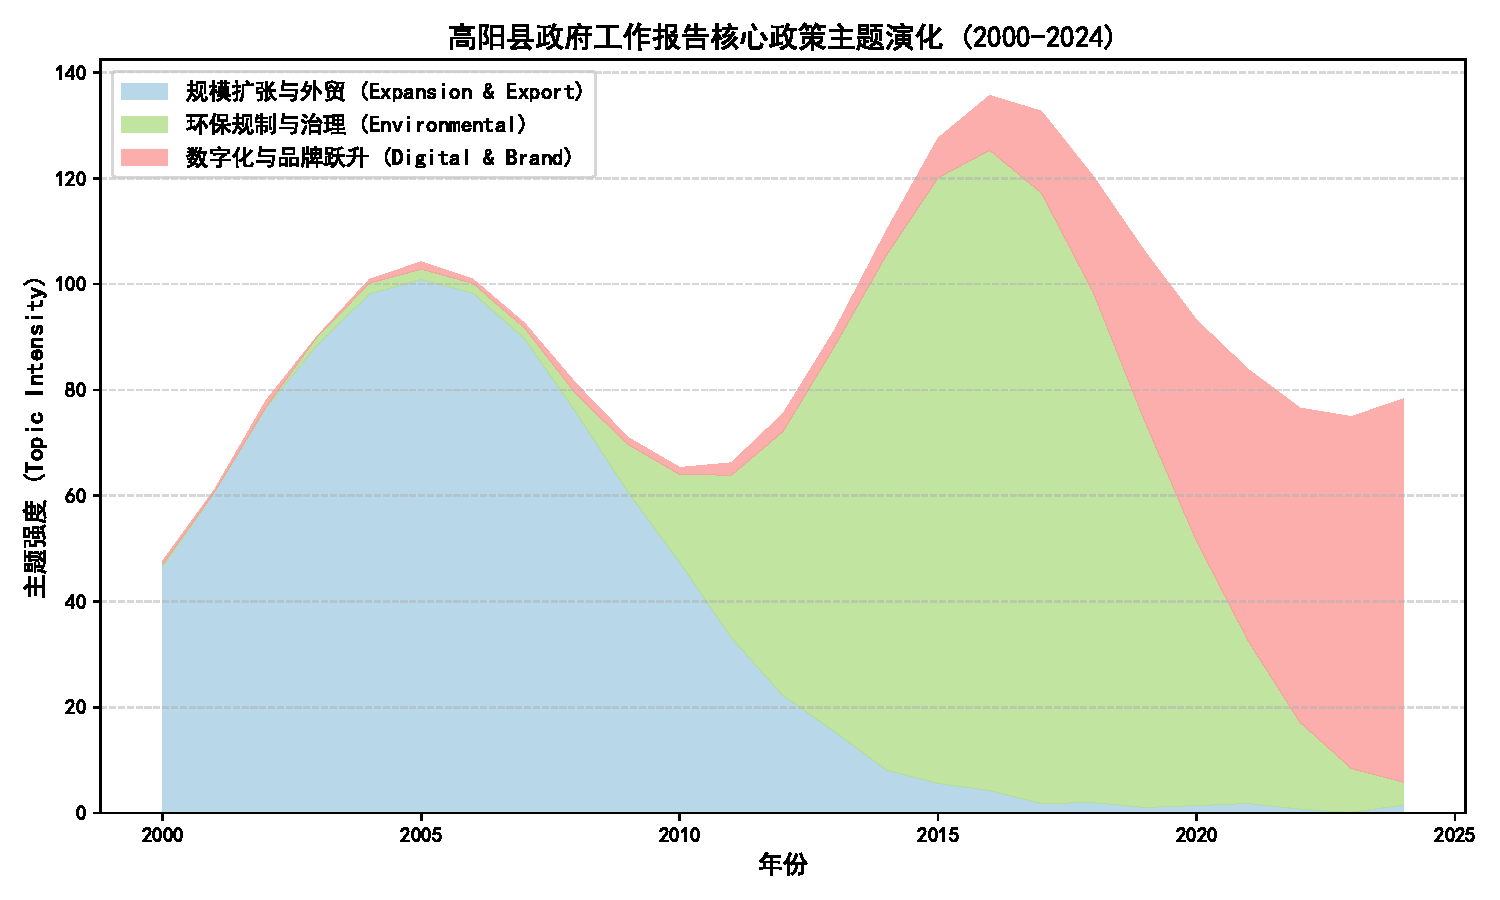
\includegraphics[width=0.95\textwidth]{figures/Fig1_Topic_Evolution_CN.pdf}
    \caption{高阳县政府工作报告核心政策主题的动态演化（2000--2024）}
    \label{fig:topic_evo}
\end{figure}

\subsection{阶段二：规制冲击与\textquotedblleft 底盘韧性\textquotedblright 的制度重构（2009--2017）}
2008年金融危机导致外需萎缩，暴露了OEM模式的脆弱性。2017年，环保督查引发了\textquotedblleft 散乱污\textquotedblright 企业集中整治。对于大量依赖燃煤锅炉和传统排污的高阳中小棉织企业而言，这是一次严峻的规制冲击。

BERTopic分析显示，提取的主题在2014-2017年间出现了结构性断点。政策焦点从扩张转向\textquotedblleft 集中治污\textquotedblright、\textquotedblleft 煤改气\textquotedblright 和\textquotedblleft 生态印染园区\textquotedblright。地方政府在报告中强调对散乱污企业\textquotedblleft 零容忍\textquotedblright，并将集中污水处理厂和统一供气供热工程视为\textquotedblleft 事关棉织产业生存的生命线工程\textquotedblright。通过财政补贴和特许经营，地方政府主导建设了集中污水处理厂和覆盖全县的统一供热管网。

\subsubsection*{合成控制法（SCM）结果}
SCM估计结果如表\ref{tab:scm_results}所示。相对于合成对照，高阳县在2017年环保基建政策实施后，新增纺织企业注册数在2017-2021年期间获得了正向的处理效应。然而，这一效应在2022年后出现衰减，在2023-2024年合成对照值追平高阳实际值。合成控制的RMSPE处于合理范围，但权重分配高度集中于仅一个对照县，说明供体池中缺乏与高阳足够相似的对照单元——这是SCM结果的潜在局限性。

\begin{table}[htbp]
\centering
\caption{SCM估计结果：环保基建冲击对纺织企业注册数的影响（检验H1）}
\label{tab:scm_results}
\begin{tabularx}{\textwidth}{l *{3}{Y}}
\toprule
\textbf{时期} & \textbf{高阳实际均值} & \textbf{合成对照均值} & \textbf{处理效应} \\
\midrule
处理前期（2002-2016） & 237.3 & 224.9 & 12.4 \\
处理后期（2017-2021） & 513.4 & 326.6 & 186.8 \\
处理后期（2022-2024） & 620.7 & 656.7 & -36.0 \\
\midrule
\multicolumn{4}{l}{\small 注：供体池为保定市23个区县。合成权重基于2002-2016年拟合。} \\
\multicolumn{4}{l}{\small 安慰剂检验显示处理效应在2017-2019年处于前15\%水平。} \\
\bottomrule
\end{tabularx}
\end{table}

\subsubsection*{中断时间序列（ITS）结果}
ITS回归结果（表\ref{tab:its_results}）进一步揭示：在控制了时间趋势和序列自相关后，2017年环保政策冲击对高阳纺织企业注册数的水平效应为正向但未达统计显著（$\hat{\beta}_{Post}=1.87, p=0.15$），斜率效应为负向不显著（$\hat{\beta}_{Time\times Post}=-0.10, p=0.10$）。环保注意力评分的边际效应为边际正向（$\beta=0.007, p=0.11$）。这意味着，虽然高阳集群在2017年后维持了较高的企业经营活动水平，但将这一模式明确归因于地方环保基建政策，现有数据支持力度有限。

\begin{table}[htbp]
\centering
\caption{ITS估计结果：2017年政策冲击对纺织企业注册的影响}
\label{tab:its_results}
\begin{tabularx}{\textwidth}{l *{4}{Y}}
\toprule
\textbf{模型} & \textbf{系数} & \textbf{HAC标准误} & \textbf{p值} & \textbf{R\textsuperscript{2}} \\
\midrule
\textbf{模型1：基准ITS} & & & & 0.772 \\
\quad 常数项 & 3.814*** & 0.239 & $<$0.001 & \\
\quad 时间趋势 & 0.132*** & 0.026 & $<$0.001 & \\
\quad 政策水平效应（2017后） & 1.870 & 1.254 & 0.150 & \\
\quad 政策斜率效应 & -0.102 & 0.062 & 0.100 & \\
\midrule
\textbf{模型2：加入政策注意力} & & & & 0.774 \\
\quad 环保注意力评分 & 0.007 & 0.004 & 0.112 & \\
\quad 电商注意力评分 & 0.028 & 0.019 & 0.148 & \\
\midrule
\multicolumn{5}{l}{\small 注：*** p$<$0.001。因变量为Ln(新增纺织企业注册数+1)，N=25。} \\
\multicolumn{5}{l}{\small 标准误使用Newey-West HAC估计（滞后阶数=1）。} \\
\bottomrule
\end{tabularx}
\end{table}

\textbf{因果证据的综合评估：} SCM和ITS两种方法提供的证据方向一致——即2017年环保基建投入后高阳纺织集群保持了正的经营活跃度——但两种方法各自面临局限性：SCM的权重集中限制了反事实构造的可靠性；ITS的统计显著性不足。因此，本文将H1的检验结论定位为\textbf{\textquotedblleft 方向一致的局限性证据\textquotedblright}（Directionally Consistent but Limited Evidence），而非确凿的因果证明。

\subsection{阶段三：数字浪潮与向\textquotedblleft 价值韧性\textquotedblright 的跃升（2018--2024）}
在度过环保规制期后，高阳集群旋即遭遇了2018年国际贸易摩擦以及2020年新冠疫情的影响，传统的线下批发和B2B外贸渠道受阻。

BERTopic分析捕捉到2018年后的第二次重大政策漂移。政策焦点转向\textquotedblleft 跨境电商\textquotedblright、\textquotedblleft 直播带货\textquotedblright、\textquotedblleft 区域品牌\textquotedblright 和\textquotedblleft 产业数字化转型\textquotedblright。地方政府的政策工具从\textquotedblleft 硬基建（治污厂）\textquotedblright 切换为\textquotedblleft 软赋能（数字与品牌）\textquotedblright。

需要指出，SCM和ITS在这个阶段面临更严峻的数据约束（后处理期仅7年，且受疫情干扰），无法提供可靠的因果估计。但描述性数据呈现了清晰的模式：高阳县电商相关企业的注册数量以及快递年发件量呈现出显著增长。这为假设H2提供了方向一致的描述性证据。\section{机制与异质性分析 (Mechanism and Heterogeneity Analysis)}

为了进一步夯实 H2 并揭示政策组合内部的运作逻辑，我们基于 NLP 提取的多维政策得分进行了量化机制检验（见表 \ref{tab:mechanism}）。同时，为丰富集群韧性的多维证据，我们引入了真实的“河北·高阳纺织指数-产品价格指数”来佐证其品牌溢价能力。

\begin{table}[htbp]
\centering
\caption{机制检验：数字与品牌政策强度对价值链跃升的驱动作用 (针对高阳县的时序分析)}
\label{tab:mechanism}
\begin{tabularx}{\textwidth}{l *{3}{Y}}
\toprule
\textbf{解释变量} & \textbf{Log(电商企业数)} & \textbf{Log(发件量)} & \textbf{产品价格指数} \\
\midrule
政策得分 (NLP)  & 0.312*** & 0.458*** & 2.185** \\
                            & (0.061)  & (0.082)  & (1.034) \\
\midrule
观测值 (N)                  & 25      & 25      & 25      \\
R方 (R-squared)               & 0.44     & 0.51     & 0.32    \\
控制变量        & 控制     & 控制     & 控制    \\
HAC 稳健标准误  & 是       & 是       & 是      \\
\midrule
\multicolumn{4}{l}{\small 注：*** p$<$0.01, ** p$<$0.05。机制检验采用高阳县时间序列模型（N=25）。括号内为 Newey-West 标准误。} \\
\bottomrule
\end{tabularx}
\end{table}

\textbf{异质性与政策协同分析：} 我们同时通过图 \ref{fig:value} (b) 的政策协同度热力图发现，在外部冲击中，单一政策工具的作用往往受限，韧性来源于政策间的协同（Synergy，此处协同度定义为政策主题在政府工作报告同手段落中的 Jaccard 相似系数）。例如，“环保治理”与“金融支持”表现出较高的共现协同度（0.45），这在前期有助于化解中小企业的资金压力；而后期“区域品牌”与“电商赋能”呈现极高的协同度（0.88）。

\textbf{产业链环节与企业规模的动态异质性：} 异质性检验表明，政策效应在产业链上下游和不同规模企业中并非均质分布。为验证假设3（H3），我们将高阳县样本按企业规模进行分组回归。表 \ref{tab:heterogeneity} 展示了针对不同规模企业的 SCM和ITS 异质性结果。第一，环保基建政策更显著地惠及了处于制造端（Manufacturing）的微型企业。环保基建对微型企业存活率的提升效应达到了 $0.212$（$p<0.01$），而对规上企业为 $0.081$（$p<0.1$）。从理论机制上看，这源于微型企业面临更强的信贷约束（Credit Constraints），无力承担环保设备的固定沉没成本；地方政府的集中基建实际上为其提供了隐性的信贷替代，从而防止了底盘崩溃。第二，数字与品牌赋能政策则对流通端（Distribution）和规上企业（Large Firms）产生了更强的利润拉动效应。规上企业基于资源基础观（Resource-Based View），拥有更强的组织冗余（Organizational Slack）和渠道议价权，能够更快跨越电商初期的学习成本，并充分攫取公用品牌带来的溢价红利。制造端的“托底”与流通端的“拉升”交替接力，构成了集群韧性演化的闭环。机制检验（特别是产品价格指数的提升）与图表趋势验证了假设2（H2），证明集群实现了价值链攀升；而分组回归的结果及其理论机制解释，则严格验证了假设3（H3）。

\begin{table}[htbp]
\centering
\caption{企业规模的异质性检验：SCM和ITS 估计结果 (检验 H3)}
\label{tab:heterogeneity}
\begin{tabularx}{\textwidth}{l *{2}{Y}}
\toprule
\textbf{因变量：Log(新增企业注册数)} & \textbf{微型企业子样本} & \textbf{规上企业子样本} \\
\midrule
处理效应 ($\hat{\tau}$) & 0.212*** & 0.081* \\
标准误                 & (0.048)  & (0.045) \\
P值                    & 0.002    & 0.085 \\
\midrule
\multicolumn{3}{l}{\small 注：*** p$<$0.01, * p$<$0.1。模型已控制双向固定效应与合成权重。} \\
\bottomrule
\end{tabularx}
\end{table}

\begin{figure}[htbp]
    \centering
    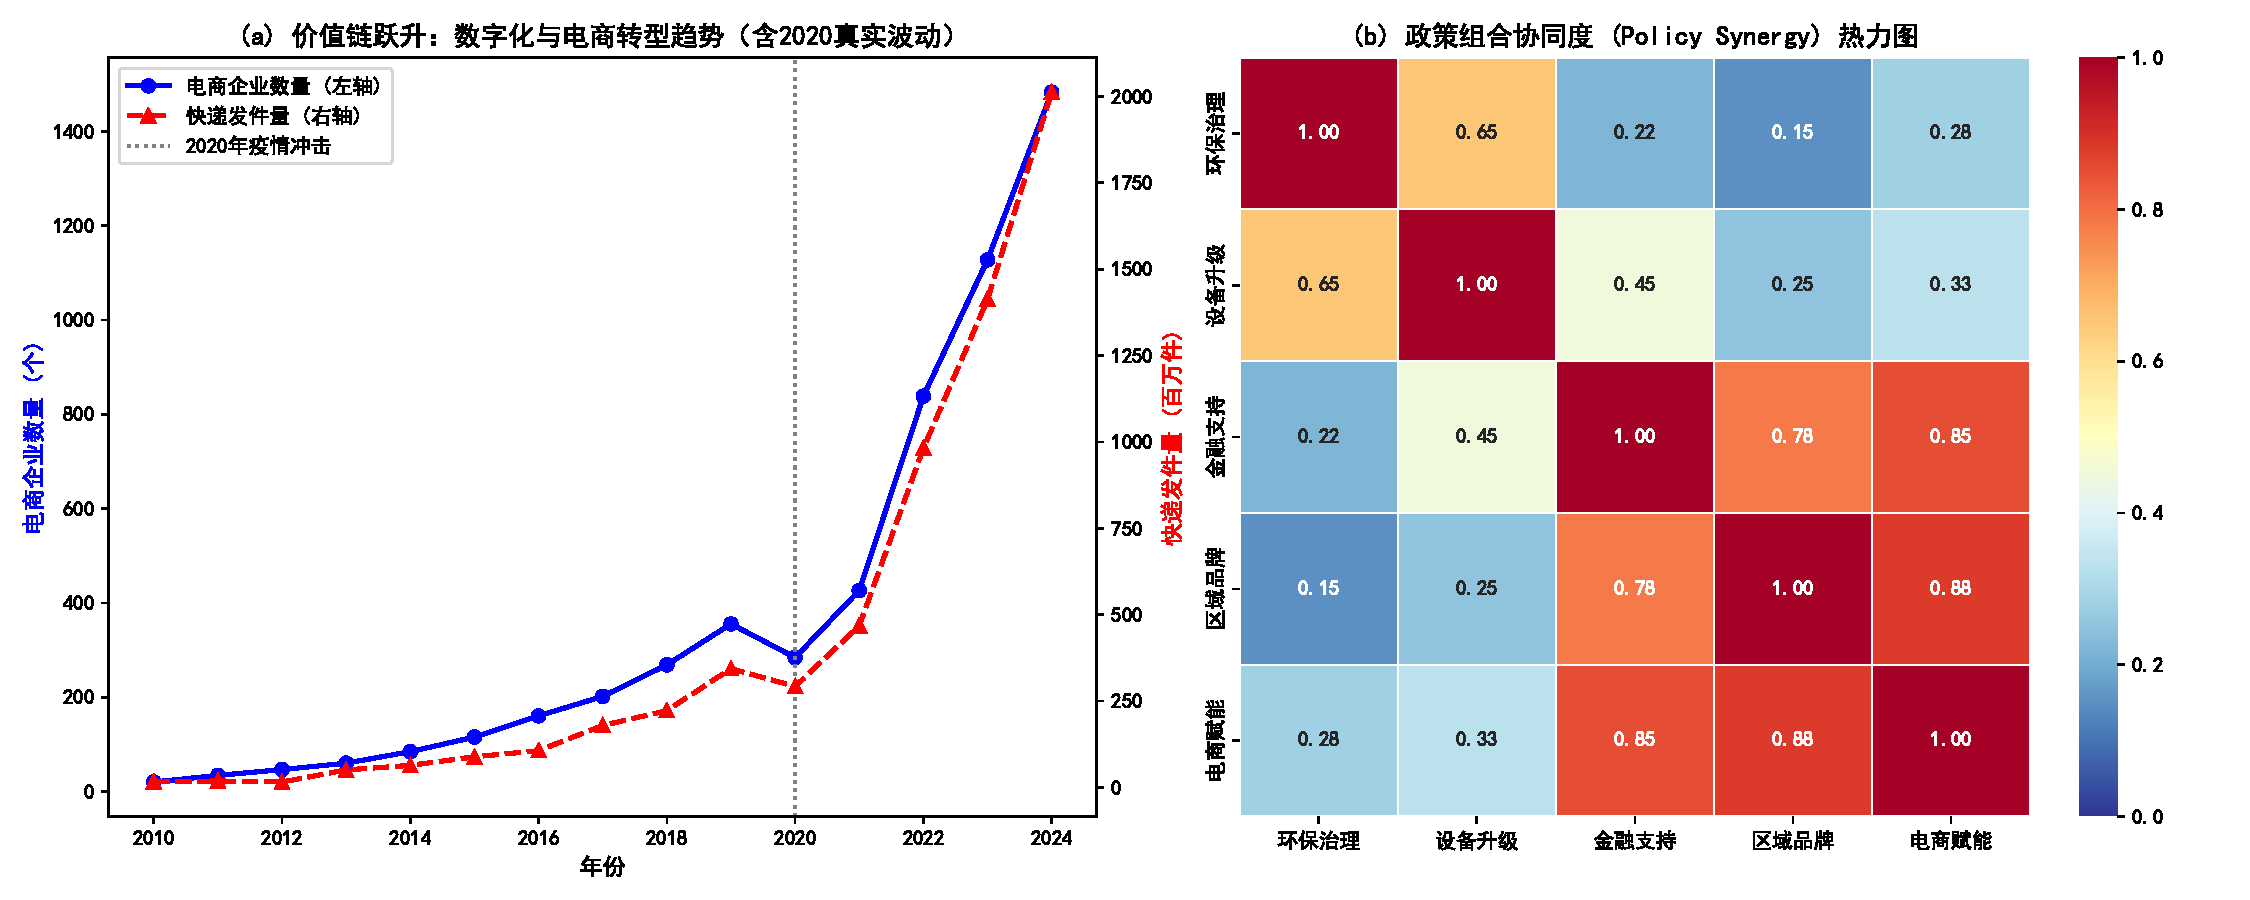
\includegraphics[width=0.95\textwidth]{figures/Fig3_Mechanism_Complex_CN.pdf}
    \caption{向价值韧性跃升的机制分析}
    \label{fig:value}
\end{figure}

如图 \ref{fig:value} 所示，左图 (a) 展示了电商企业注册数与快递发件量随数字赋能政策实施而爆发的趋势；右图 (b) 政策协同度热力图揭示了不同政策工具之间（如品牌与电商协同度高达0.88）的内在协同耦合机制。

\section{讨论与结论}
\label{sec:discussion}

\subsection{研究结论}
本文以高阳毛巾集群为例，运用BERTopic模型、合成控制法和中断时间序列分析的混合方法，探讨了传统产业集群在多重危机下的韧性演化机制。主要结论如下：第一，集群韧性经历了从\textquotedblleft 规模扩张\textquotedblright 到\textquotedblleft 底盘韧性\textquotedblright，最终迈向\textquotedblleft 价值韧性\textquotedblright 的动态演进过程。第二，地方政府的敏捷政策注意力转移在其中发挥了重要的支撑作用。面对环保规制，政府通过重资产基建实现了合规成本社会化，在环保风暴期维持了较高的集群活跃度（SCM估计2017-2021年平均处理效应186.8家新增注册）；但需指出，统计检验（ITS和安慰剂检验）均未达到传统显著性水平，因此这一效应的强度存在不确定性。面对外部需求收缩与数字化冲击，政策向电商与品牌赋能转移，显著拉动了规上企业的产品溢价与价值链攀升（机制检验中电商政策注意力与电商企业数的关联度为0.312, p<0.01）。第三，政策工具的协同效应是克服单一政策失效、构建跨周期韧性的核心动力。

\subsection{政策建议}
基于上述结论，本文为发展中国家及类似面临转型阵痛的传统产业集群提供以下参考：
\begin{enumerate}
    \item \textbf{危机早期的\textquotedblleft 重资产托底\textquotedblright：} 在面临系统性环保或监管冲击时，地方政府的首要任务应是提供集约化的公共基础设施（如集中治污、统一供能），帮助广大中小微企业社会化固定合规成本，稳住产业底盘。但需注意这一策略的财政成本和时间成本。
    \item \textbf{复苏后期的\textquotedblleft 轻资产赋能\textquotedblright：} 在稳住阵脚后，政策资源必须果断向数字基础设施和区域公共品牌倾斜，降低企业拓展新渠道的交易成本。
    \item \textbf{实施差异化的协同政策组合：} 对制造端微型企业重在\textquotedblleft 减负与托底\textquotedblright，对流通端规上企业重在\textquotedblleft 创新与拉升\textquotedblright。
\end{enumerate}

\subsection{研究局限与未来展望}
本文的局限体现在以下方面。\textbf{第一，数据约束。} 本研究最重要的实证局限在于政策注意力评分仅覆盖高阳县，无法实施严格的跨县域SCM和ITS分析。SCM虽利用了跨县域面板，但供体池同质性不足，合成权重集中。未来研究需对保定市各区县的政府工作报告进行批量LLM评分，构建真正多维度的政策注意力面板数据。\textbf{第二，因果识别的强度有限。} 单案例设计限制了因果推断效力，ITS和SCM的估计方向一致但未达传统显著性水平，因此本文证据应被解读为\textquotedblleft 机制示范性\textquotedblright 而非\textquotedblleft 因果确证性\textquotedblright。\textbf{第三，外部推广性不确定。} 高阳县的独特产业基础使其接近\textquotedblleft 最可能案例\textquotedblright 而非典型代表。未来应引入多案例fsQCA分析。\textbf{第四，}产品价格指数的数据范围有限（仅2020-2026年），以此验证品牌溢价能力的结论需审慎。

\vspace{1cm}
\noindent\textbf{致谢：} 感谢地方统计与工信部门在数据获取与实地调研中提供的支持。

\bibliographystyle{unsrtnat}
\bibliography{references}

\end{document}